\documentclass[10pt]{article}
\usepackage{braket}
\usepackage{algorithm}
\usepackage{algpseudocode}
\usepackage{soul}
\usepackage{float}
\usepackage{tabularx}
\usepackage{mathtools}
\usepackage{amsmath, amssymb, amsthm}
\usepackage{tikz}
\usetikzlibrary{arrows}
\usetikzlibrary{decorations.text}
\usepackage{enumitem}
\usepackage{geometry}
\usepackage{fancyhdr}
\usepackage{titlesec}
\usepackage{xltabular}
\usepackage{color}
\usepackage{hyperref}
\geometry{margin=1in}

\pagestyle{fancy}
\fancyhf{}
\cfoot{\thepage}
\title{SFWRENG 3DX4 - Pre-lab 2}
\author{Matthew Farah, \href{mailto:farahm11@mcmaster.ca}{$\langle$farahm11@mcmaster.ca$\rangle$}, 400468251}
\date{\today}

\hypersetup{
	colorlinks=true,
	linkcolor=blue,
	filecolor=magenta,
	urlcolor=blue,
	citecolor=blue,
	anchorcolor=blue
}

\fancyhead{}
\fancyhead[L]{Matthew Farah, \href{mailto:farahm11@mcmaster.ca}{$\langle$farahm11@mcmaster.ca$\rangle$}, 400468251}
\fancyhead[R]{SFWRENG 3DX4 - Pre-lab 2}

\AtBeginEnvironment{align}{\setcounter{equation}{0}}

\newcommand{\comment}[1]{\parbox[t]{0.45\textwidth}{\raggedright #1}}

\setlength{\parindent}{0cm}

\setcounter{tocdepth}{3}
\hypersetup{bookmarksopen=true, bookmarksopenlevel=2, bookmarksdepth=3}

\newcounter{question}
\renewcommand{\thequestion}{\arabic{question}}

\newenvironment{question}{
	\refstepcounter{question}
	\phantomsection
	\addcontentsline{toc}{section}{\protect{\large{Question \thequestion}}}
	\vspace{1em}
	\par
	\large\textbf{Question \thequestion}
	\vspace{.2cm}
	\par
	\setcounter{subquestion}{0}
	\setcounter{step}{0}
}{\vspace{.5em}}

\newenvironment{solution}{
	\vspace{1em}\par\large\textbf{{Solution:}}\par\vspace{1em}
}{
	\vspace{1em}
	\newpage
}

\newcounter{subquestion}
\renewcommand{\thesubquestion}{\alph{subquestion}}

\newenvironment{subquestion}{
	\refstepcounter{subquestion}
	\phantomsection
	\vspace{1em}\par\large\textbf{(\thesubquestion)}\hspace{-.5em}
	\setcounter{step}{0}
	\addcontentsline{toc}{subsection}{\protect{\large{Part \thequestion.\thesubquestion}}}
}{
	\par
	\vspace{1em}
}

\makeatother

\makeatletter

\newcounter{step}
\renewcommand{\thestep}{\Roman{step}}

\newenvironment{step}{
	\refstepcounter{step}
	\vspace{1.5em}\par\noindent\large\textbf{(\thestep)}
}{
	\par
	\vspace{1.5em}
}

\makeatother

\newcolumntype{Y}{>{\centering\arraybackslash}X}
\renewcommand{\arraystretch}{1.8}

\fontsize{10pt}{14pt}\selectfont

\begin{document}

\maketitle

\tableofcontents
\newpage

\begin{question}
	Once again, our first order approximation of the transfer function of a DC electric
	motor with respect to angular velocity is

	\begin{gather*}
		G_{\omega} = \frac{\Omega(s)}{V(s)} = \frac{A}{\tau{s} + 1} \\
	\end{gather*}

	Where $A$ and $\tau$ are positive, real-valued constants. $\Omega(s)$ and $V(s)$ are angular velocity
	and voltage as functions of $s$ in the Laplace domain. (Note: $\Omega$ is capital $\omega$ so we are
	using $\Omega(s) := L\set{\omega(t)}$.) \\

	We will now develop a formula for the motor DC gain constant $A$ in terms of a
	step input change $\Delta{V}$ and step output change $\Delta{\omega}$.
\end{question}

\begin{subquestion}
	Using the final value theorem, find an expression for the steady state value
	of $\omega(t)$ when a step input of amplitude $V_{x}$ is applied. NOTE: $\tau > 0$ so the
	pole of $G_{\omega}(s)$ at $s = \frac{-1}{\tau}$ is in the open Left Half Plane (LHP) so the system
	is stable! Therefore, we can use the final value theorem.
\end{subquestion}

\begin{solution}
	We know that the steady state vale of $\omega(t)$ is given by $\lim_{t\to\infty}\omega(t)$. By the final value theorem, we know that $\lim_{t\to\infty}\omega(t) = \omega(\infty) = \lim_{s\to{0}}s\Omega(s)$. Since $\frac{\Omega(s)}{V(s)} = \frac{A}{\tau{s} + 1}$, we therefore know that:

	\begin{align*}
		\Omega(s) &= \frac{AV(s)}{\tau{s} + 1} \\
	\end{align*}

	And so:

	\begin{align*}
		s\Omega(s) &= \frac{sAV(s)}{\tau{s} + 1} \\
	\end{align*}

	Now, note that a step input of amplitude $V_{x}$ is given by $V_{x}{u(t)}$. By the linearity of the Laplace transform and the lookup table, we have that $\mathcal{L}\set{V_{x}u(t)} = \frac{V_{x}}{s}$, so:

	\begin{align*}
		s\Omega(s) &= \frac{sA{V_{x}}}{s(\tau{s} + 1)} \\
		&= \frac{A{V_{x}}}{\tau{s} + 1} \\
	\end{align*}

	Hence:

	\begin{align*}
		\lim_{s\to{0}}s\Omega(s) &= \lim_{s\to{0}}\frac{A{V_{x}}}{\tau{s} + 1} \\
		&= \frac{A{V_{x}}}{\tau(0) + 1} \\
		&= \frac{A{V_{x}}}{1} \\
		&= A{V_{x}} \\
	\end{align*}
\end{solution}

\begin{subquestion}
	Give the expression for $\omega(t)$ in response to a step input $V_{x}$ at time $t = 0$.
	Assume a non-zero initial condition for $\omega(t)$, i.e., $\omega(0) = \omega_0$. Note that
	the response due to a non-zero initial condition $\omega_{0}$ can be modeled as the
	response due to input $v(t) = \omega_{0}\delta(t)$ where $\delta(t)$ in the impulse function. Since
	$G_{\omega}(s)$ is a linear system, the response to step input $V_{x}$ with non-zero initial
	condition $\omega_{0}$ is just the sum of the responses due to the step and the initial
	condition.
\end{subquestion}

\begin{solution}
	To find an expression for $\omega(t)$, we must find $\mathcal{L}^{-1}\set{\Omega(s)}$. Since we are given that $\omega(0) = \omega_{0}$ is non-zero, we can use the linearity of the transfer function $G_{\omega}(s)$ to find $\Omega(s)$. Since the input to the system $v(t)$ including both the initial condition and step input can be represented by:

	\begin{align*}
		v(t) &= \delta(t)\omega_{0} + V_{x}u(t) \\
	\end{align*}

	We can use the linearity of the Laplace transform, our given conversion table, and the definition of the Dirac-delta function ($\delta(t)$) to conclude that:

	\begin{align*}
		V(s) &= \omega_{0} + \frac{V_{x}}{s} \\
	\end{align*}

	Therefore, we have that:

	\begin{alignat*}{3}
		G_{\omega}(s) &= \quad \frac{\Omega(s)}{V(s)} &= \frac{A}{\tau{s} + 1} \\\\
		&= \frac{\Omega(s)}{\omega_{0} + V_{x} / {s}} \; &= \frac{A}{\tau{s} + 1} \\\\
	\end{alignat*}

	And so:

	\begin{align*}
		\Omega(s) &= \frac{A(\omega_{0} + V_{x} / s)}{\tau{s} + 1} \\\\
		&= \frac{A\omega_{0}}{\tau{s} + 1} + \frac{A{V}_{x}}{s(\tau{s} + 1)} \\\\
		&= \frac{A\omega_{0}}{\tau} \left( \frac{1}{s + 1 / \tau} \right) + A{V}_{x} \left( \frac{1}{s(\tau{s} + 1)} \right) \\
	\end{align*}

	Using linearity and the conversion table we are able to find the inverse Laplace of the term on the left. However, we must perform partial fraction decomposition on the rightmost term before we are able to take the inverse Laplace of $\Omega(s)$. Therefore, let $B, C$ be constants we will soon find such that:

	\begin{align*}
		\frac{1}{s(\tau{s} + 1)} &= \frac{B}{s} + \frac{C}{\tau{s} + 1} \\
	\end{align*}

	We therefore know that:

	\begin{align*}
		1 &= B(\tau{s} + 1) + C{s} \\
		&= B\tau{s} + B + C{s} \\
	\end{align*}

	By equating coefficients, we can clearly see that $B = 1$, implying that $C = -\tau$. Substituting back into our original equation, we therefore have that:

	\begin{align*}
		\Omega(s) &= \frac{A\omega_{0}}{\tau} \left( \frac{1}{s + 1 / \tau} \right) + A{V}_{x} \left( \frac{1}{s} - \frac{\tau}{\tau{s} + 1} \right) \\\\
		&= \frac{A\omega_{0}}{\tau} \left( \frac{1}{s + 1 / \tau} \right) + AV_{x} \left(\frac{1}{s} \right) - AV_{x}\tau \left( \frac{1}{\tau{s} + 1} \right) \\\\
		&= \frac{A\omega_{0}}{\tau} \left( \frac{1}{s + 1 / \tau} \right) + AV_{x} \left(\frac{1}{s} \right) - \frac{AV_{x}\tau}{\tau} \left( \frac{1}{s + 1 / \tau} \right) \\\\
		&= \frac{A\omega_{0}}{\tau} \left( \frac{1}{s + 1 / \tau} \right) + AV_{x} \left(\frac{1}{s} \right) - AV_{x} \left( \frac{1}{s + 1 / \tau} \right) \\
	\end{align*}

	And so, using the linearity of the inverse Laplace and the conversion table, we can conclude that:

	\begin{align*}
		\omega(t) &= \frac{A\omega_{0}}{\tau}e^{-\frac{1}{\tau}t} + AV_{x}u(t) - AV_{x}e^{-\frac{1}{\tau}t} \\\\
		&= \frac{A(\omega_{0} - V_{x}\tau)}{\tau}\left(e^{-\frac{1}{\tau}t} \right) + AV_{x}u(t) \\
	\end{align*}
\end{solution}

\begin{subquestion}
	For $\omega(t)$ you computed in 1.b.), what is $\lim_{t\to\infty}$? How does it compare
	to your answer from 1.a.)?
\end{subquestion}

\begin{solution}
	Since $\tau > 0$, we know $-\frac{1}{\tau} < 0$ and hence:

	\begin{align*}
		\lim_{t\to\infty}\omega(t) &= \lim_{t\to\infty} \frac{A(\omega_{0} - V_{x}\tau)}{\tau}\left(e^{-\frac{1}{\tau}t} \right) + AV_{x}u(t) \\\\
		&= \frac{A\omega_{0}}{\tau}\left( 0 \right) + AV_{x}(1) \\\\
		&= AV_{x} \\\\
	\end{align*}

	This is identical to the result obtained in 1.a.), implying that the initial state of $\omega(t)$ at $t = 0$ has no impact on the steady state value of $\omega(t)$ when the system's input is the same step function.
\end{solution}

\begin{subquestion}
	Now assume that you run the motor with an initial step input of $V_{min}$ until
	time $t_0$ when the system has reached steady state before the step input is
	changed to $V_{max}$. In other words, your system input will take the form:

	\begin{align*}
		v(t) &= \begin{cases}
			V_{max}, \; t \ge t_0 \\
			V_{min}, \; 0 \le t < t_0 \\
		\end{cases}
	\end{align*}

	Where $t_0 >> \tau$ and $V_{min}$ and $V_{max}$ may be non-zero. Use the results above to show that:

	\begin{align*}
		A = \frac{\Delta{\omega}}{\Delta{V}} \\
	\end{align*}

	Where:
	\begin{itemize}
		\item $\Delta{V} = V_{max} - V_{min}$
		\item $\Delta{\omega} = \omega_{ss} - \omega_0$, where $\omega_0$ is the steady state response to a constant input $V_{min}$ and $\omega_{ss}$ is the steady state response to the input $V_{max}$.
	\end{itemize}
\end{subquestion}

\begin{solution}
	By questions 1.a.), we know that:

	\begin{align*}
		\omega_0 &= AV_{min} \\
	\end{align*}

	And:

	\begin{align*}
		\omega_{ss} &= AV_{max} \\
	\end{align*}

	Which means:

	\begin{align*}
		\omega_{ss} - \omega_0 &= AV_{max} - AV_{min} \\
		&= A(V_{max} - V_{min}) \\
	\end{align*}

	And hence:

	\begin{align*}
		A &= \frac{\omega_{ss} - \omega_0}{V_{max} - V_{min}} \\\\
		&= \frac{\Delta{\omega}}{\Delta{V}}
	\end{align*}
\end{solution}

\begin{question}
	Using the formula derived in question 1, use the following graphs to calculate
	$A$ for this system.

	\begin{figure}[htbp]
		\centering
		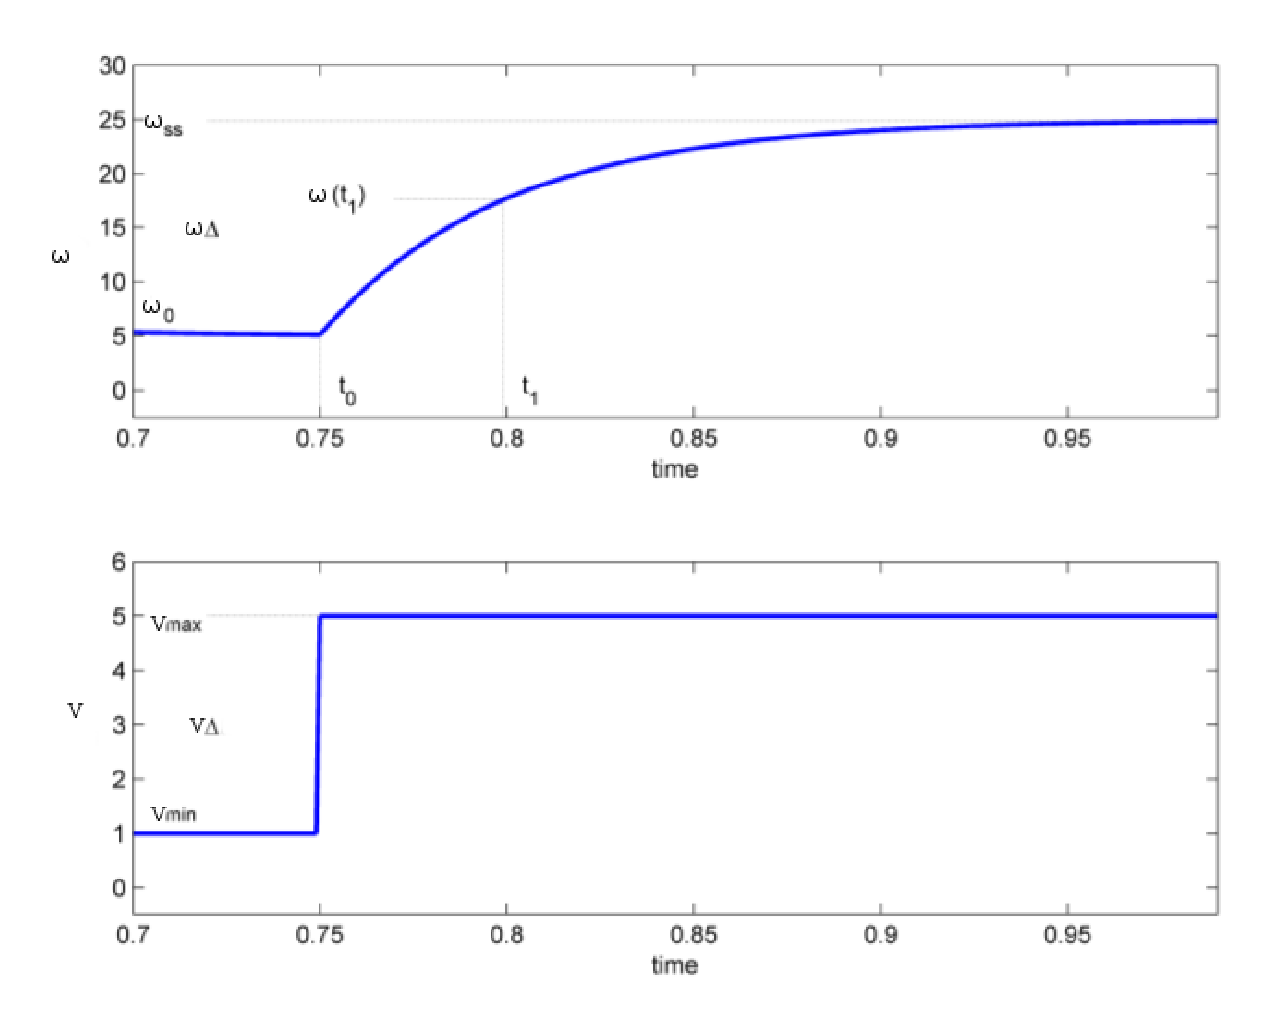
\includegraphics[width=\textwidth]{./imgs/Question-2.png}
		\caption{A First Order Response to Step Input}
	\end{figure}
\end{question}

\begin{solution}
	From the graph, we can clearly observe that $\Delta{\omega} = 20$ and $\Delta{V} = 4$. Thus, using the formula developed in 1.d.), we have:

	\begin{gather*}
		A = \frac{\Delta{\omega}}{\Delta{V}} = \frac{20}{4} = 5 \\
	\end{gather*}
\end{solution}

\begin{question}
	For a first order system, the time it takes a step response to reach 63.2\% of its
	steady state value ($t_1 - t_0$ in Fig. 1) is the response's time constant $\tau$ . i.e., at
	time $t_1$, $\omega(t_1) = 0.632\Delta{\omega} + \omega_0$. Find the time constant $\tau$ for the above system
	in Fig. 1.
\end{question}

%TODO: Complete
\begin{solution}
	Since $\tau$ represents the time the system needs to reach 63.2\% of its steady state value, and since we know that the system's steady state value is evidently 25 from observing the graph, we know $$

	\begin{align*}
		\tau = t_1 - t_0 \\
		\omega(t_1) = .632\Delta{\omega} + \omega_0
		&= .632{20} + 5
		&= 17.64
	\end{align*}

\end{solution}

%TODO: Complete
\begin{question}
	Using $A$ and $\tau$, give the transfer function $G_{\omega}(s)$ in terms of $s$.
\end{question}

\begin{solution}

\end{solution}

%TODO: Complete
\begin{question}
	Complete problem 21(a) in Chapter 4 of Control Systems Engineering 8th ed:

	For the unit step response shown, find the transfer
	function of the system.

	\begin{figure}[htbp]
		\centering
		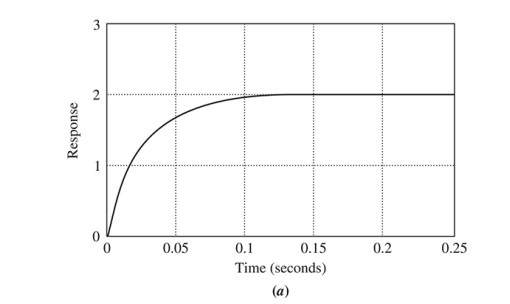
\includegraphics[width=\textwidth]{./imgs/Question-5.png}
		\caption{System response to step input}
	\end{figure}
\end{question}

\begin{solution}

\end{solution}

%TODO: Complete
\begin{question}
	In one or two paragraphs, describe a situation in which it is
	preferable to derive a transfer function experimentally, and then
	design/calibrate a controller using simulation software, rather than
	experimenting with the plant to design/calibrate the controller
	directly. Describe a situation in which this is not preferable. (Answer
	in complete sentences!)
\end{question}

\begin{solution}

\end{solution}

































\end{document}
